\documentclass{article}
\usepackage[spanish]{babel}
\usepackage[T1]{fontenc}
\usepackage[ansinew]{inputenc}
\usepackage{graphicx}
\usepackage{url}
\usepackage[maxbibnames=99, sorting=none, backend=bibtex]{biblatex}
\addbibresource{bibpr2sim.bib}

\begin{document}
\title{\textbf{Diagramas Voronoi}}
\author{Clara T\'ellez}
\maketitle

\section{Objetivo}\label{obj}

 La pr\'actica consite en examinar de manera sistem�tica el efecto del n�mero de semillas y del tama�o de la zona en la distribuci�n de los largos de las grietas que se forman  en los diagramas Voronoi \cite{eli}.

\section{Metodolog\'ia}\label{met}

Para examinar los efectos del tama�o del diagrama y el n\'umero de semillas sobre los largos de las grietas y hacer el respectivo tratamiento estad\'istico se us\'o R en su versi\'on 3.6.2.


La rutina se dise�\'o variando el tama�o del diagrama inicial, con rejillas de 30 x 30, 40 x 40 y 50 x 50, y tambi\'en el n\'umero de semillas (5, 10 y 15).  posteriormente se provocaron grietas con una propagaci\'on preferencial hacia los bordes de frontera y se calcul\'o el largo de las mismas.

Para cada modelo se realizaron cien r\'eplicas.  A partir de estos datos se hizo un an\'alisis de varianza y se muestran los datos en diagrama de cajas y bigotes.


\section{Resultados y Discusi\'on}\label{res}

A partir de los datos se construy\'o un diagrama de cajas y bigotes (figura \ref{f1}) en el que se muestra el largo de las grietas con respecto al tama\'no de la rejilla.  A simple vista no se aprecia mayor diferencia, sin embargo, al realizar la ANOVA (cuadro\ref{t1}), el an\'alisis estad\'istico muestra una significancia menor a 0.05 por lo que se rechaza la hip\'otesis nula y se puede afirmar que existen diferencias significativas al variar los tama\'nos y las semillas en los diagramas Voronoi.



\begin{figure}
  \begin{center}
    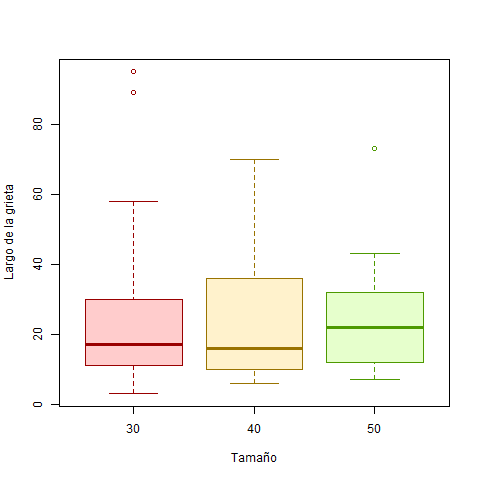
\includegraphics[width=10cm]{boxplot.png}
  \end{center}
  \caption{Largo de la grieta por tama\'no }
  \label{f1}
\end{figure}



\begin{table} 
 \caption{Comparaci\'on del largo de las grietas con relaci\'on al tama\'no de la rejilla y al n\'umero de semillas}
 \label{t1}
 \begin{center}
 \begin{tabular}{rrrrrr}
\texttt{} & \texttt{GL} & \texttt{Suma Cuad.} &\texttt{Media Cuad.} & \texttt{F}  & \texttt{Pr(>F)} \\
Tama\'no & 2 & 3127 & 1563.7 & 3.941 & 0.0233 \\ 
Semillas  & 2 & 1819 & 909.5 & 2.292 & 0.0107\\ 
Tama\'no;Semillas & 4 & 988 & 246.9 & 0.622 & 0.0448 \\ 
Residuales & 81 & 32142& 396.8 \\ 
\end{tabular}
\end{center}
\end{table}


\section{Conclusiones}\label{con}   

El tama\'no y el n\'umero de semillas afectan el largo de las grietas que se producen en los diagramas Voronoi.
\printbibliography
\end{document}